%************************************************************************************
% Authors: Martin Nordio
% Date: March 2011
% Root file: report_root.tex
%************************************************************************************


%----------------------------------------------------------------------------
\chapter{User Guide}\label{userguide}
%----------------------------------------------------------------------------





\section{Setup and Run Client}

The fastest way to get started with CloudStudio is to use a precompiled client JAR directly from GitHub.

\begin{itemize}

\item Download the latest \texttt{CSClient.jar} directly from: \newline \texttt{http://github.com/fgremper/CloudStudio}

\item Go to \texttt{http://cloudstudio.ethz.ch:7330/} and create a new account by clicking "Sign up" in the top right corner and providing a new username and password.

\item Create a new config.xml file in the same directory as the client JAR you downloaded and paste in the setup configuration.

\item Replace the username and password with your username and password you just created.

\item If you want to work with an existing CloudStudio project, provide its repository alias and the path to your local Git repository, and make sure the repository owner adds you to the repository access list.

\item If you want set up a new CloudStudio project, click "Create repository" in the repository overview and provide an alias, description and possible an URL to a remote repository. Use the repository alias in your configuration file.

\item You can use the client to monitor multiple repositories with the same CloudStudio user account.

\end{itemize}

\section{Using the Web Interface}\label{webinterfaceguide}



This section quickly guides you through the different views in the CloudStudio web interface and shows you how to use them.


\section{Login}

This is the initial view of the CloudStudio web interface. Log in with your credentials or choose to sign up for a new account in the top-right corner.





\begin{figure}[h!]
  \centering
  \fbox{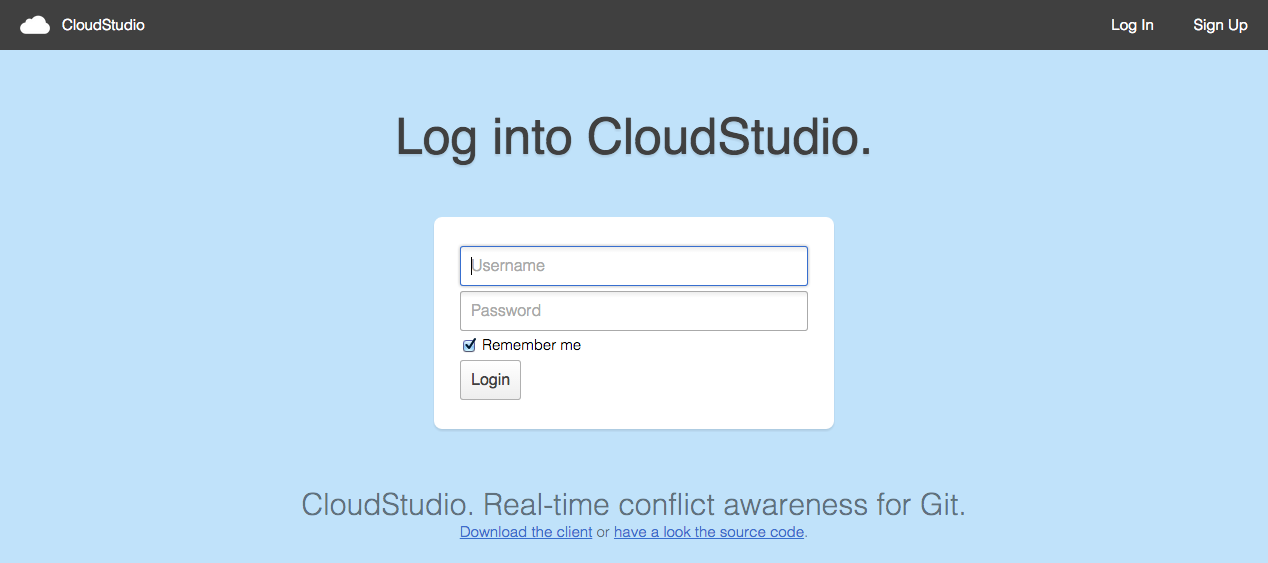
\includegraphics[width=0.9\textwidth]{login}}
  \caption{Web interface login page}
  \label{fig:login}
\end{figure}



\section{Repository Overview}

The $Repository$ $Overview$ is the main view after you log into the web interface. It provides a list of all repositories you have access to. \\

If you have administrator privileges or are the repository owner, you can add or remove users from the project, as well as change the repository URL (path to a remote, e.g. GitHub) or description, by clicking the $Edit$ button in the top-right corner of a repository. If you have repository creation privileges, you can create a new CloudStudio repository by clicking the $Create$ $repository$ button at the top. \\

Click on a repository to step into the branch level awareness view.



\begin{figure}[h!]
  \centering
  \fbox{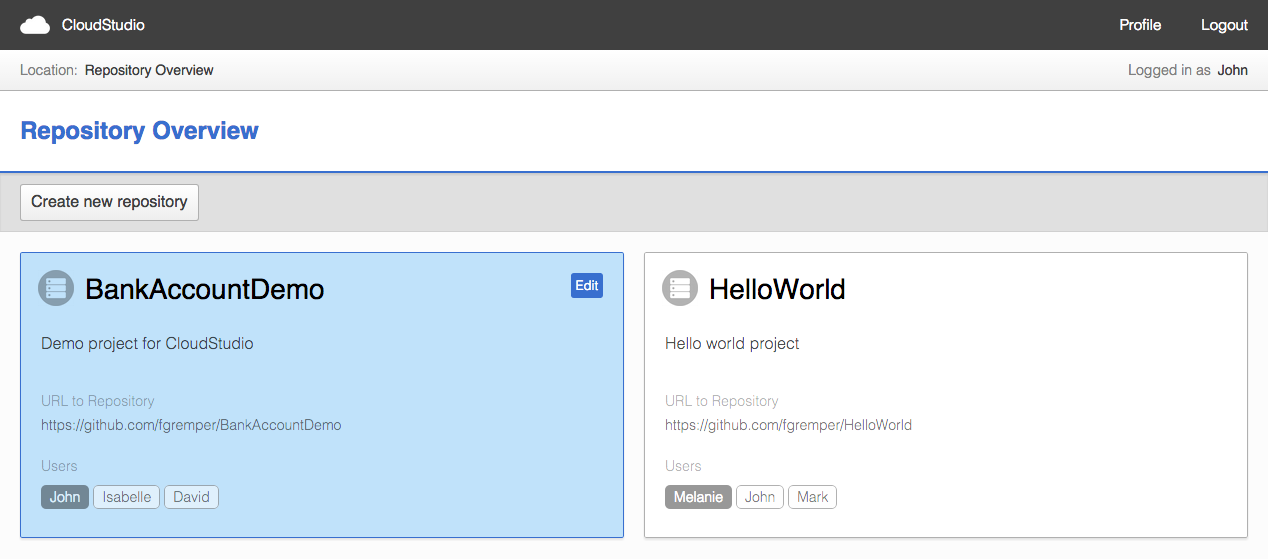
\includegraphics[width=0.9\textwidth]{overview}}
  \caption{Web interface repository overview}
  \label{fig:overview}
\end{figure}





\section{Branch Level Awareness}

In this view, we are interested in the branch pointers of all users in relation to the branch pointers of the origin. \\

Assume we are looking at the master branch. If a user's master branch reference points to the same commit as on the origin, then the users relationship is given as "Up to date". If the user has made a new commit locally but hasn't pushed it to the server yet, the user is displayed under "Made new commits". If someone else has pushed a new commit to the origin after our user has last pulled from the origin, the user is listed under "Behind origin". \\

Local branches that have not been pushed to the origin are given as "Local branch"; if a user has not fetched a given branch, it is displayed as "Remote branch". \\

Users listed under "Working On This Branch" have currently checked out this branch locally. The time since the last time the CloudStudio Client has been run is given next to the username in brackets. On the top-right you can also see when information from the central repository has last been retrieved. \\

Clicking on a branch takes you to the file level awareness view for a given branch.



\begin{figure}[h!]
  \centering
  \fbox{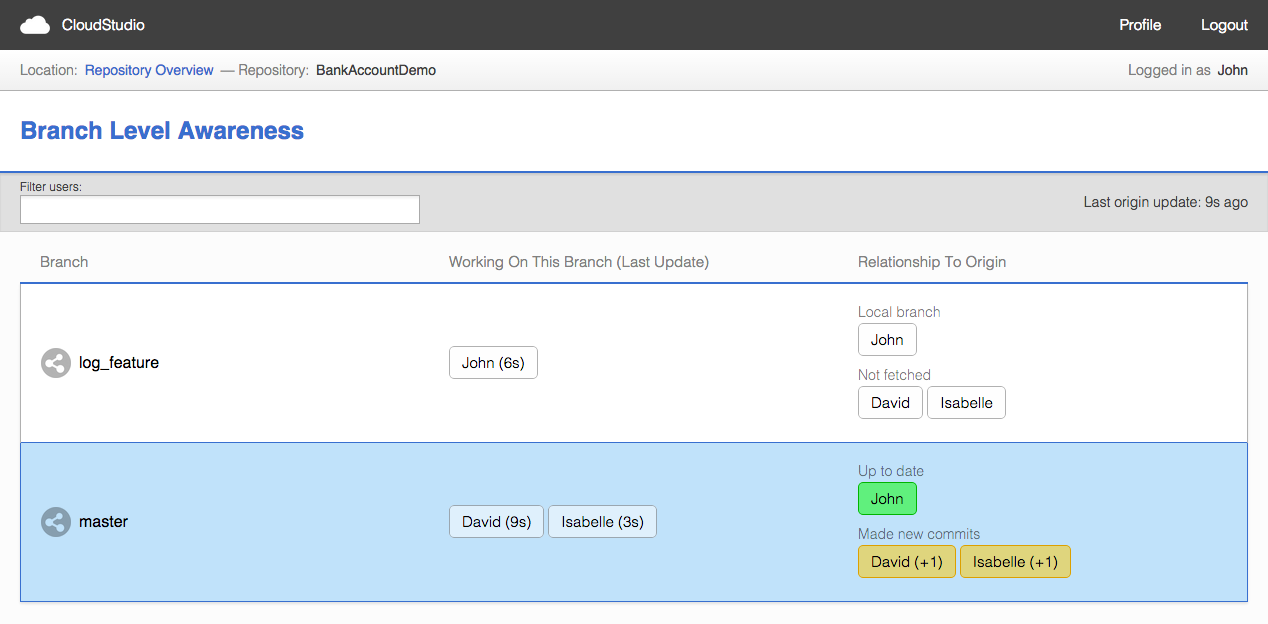
\includegraphics[width=0.9\textwidth]{branchlevel}}
  \caption{Web interface branch level awareness}
  \label{fig:branchlevel}
\end{figure}





\section{File Level Awareness}

For each file in a branch, file conflicts between you and every other user are displayed. A file conflict occurs when two files aren't identical and is highlighted in yellow. In red, content conflicts are displayed---a content conflict occurs if a merge of two files would result in a merge conflict. This feature uses a three-way comparison approach with a common ancestor of the two files as a merge-base in order to mimic the functionality of a Git merge. \\

By selecting the $view$ $as$ $origin$ at the top, instead of comparing your files to those of all others, the files of the origin are taken as the base for comparison. Various filters let you selectively show or hide users, enable or disable the content conflict feature, view the latest uncommitted versions of files or deal with contents of files that have already been locally committed. \\

Folders act as groups and the conflict status of files are propagated upwards. If at least one file in a folder is red, the parent folder becomes red and the user responsible for the content conflict is shown. Likewise, if there are file conflicts in a folder but no content conflicts, the enclosing folder becomes yellow. This functionality is especially useful if your project is setup in subfolders for different features. \\

The comparison branch refers to the branch that you compare your files to. This is useful if you know that the branch you're working in is going to be merged into another branch soon and want to see what conflicts would occur. \\

By clicking on a user you can step into the content awareness view, that lets you view the differences between the two of you.



\begin{figure}[h!]
  \centering
  \fbox{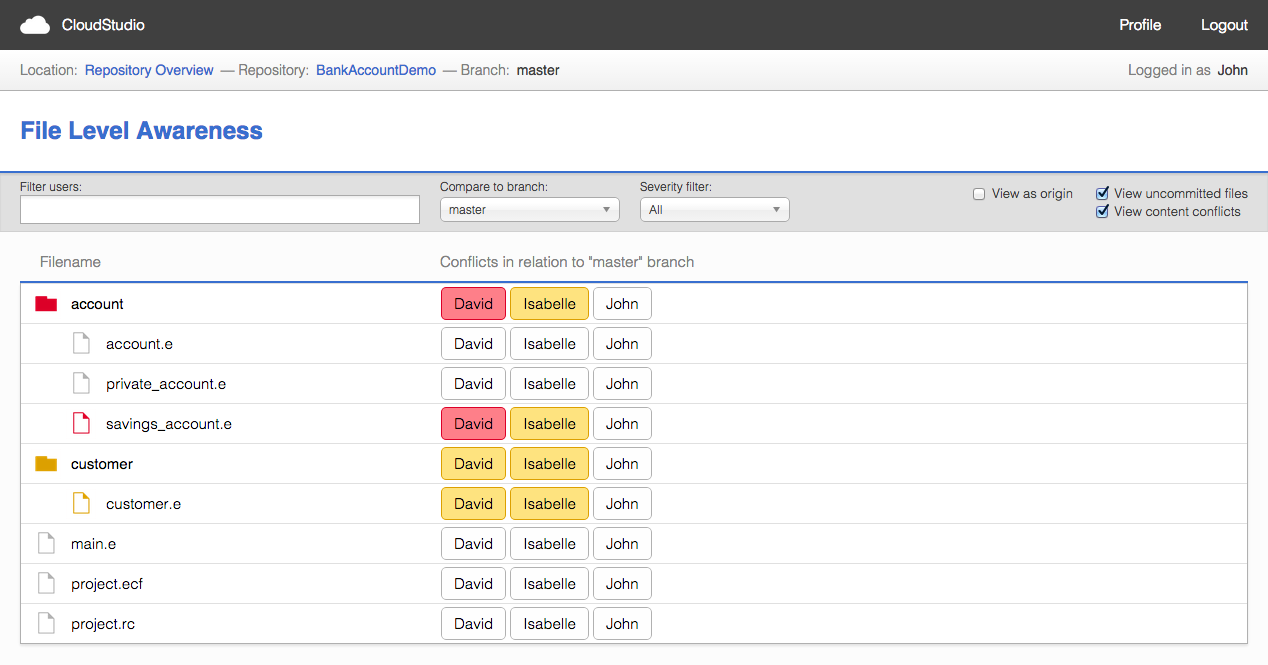
\includegraphics[width=0.9\textwidth]{filelevel}}
  \caption{Web interface: file level awareness}
  \label{fig:filelevel}
\end{figure}



\section{Content Awareness}

In this view, two files are compared side-by-side. Without checking the $show$ $conflicts$ options, files are compared directly to each other and the differences are highlighted. \\

When you choose to $show$ $conflicts$, a common ancestor of the two files is used as a merge-base to create a three-way comparison. Per definition, a conflict occurs when three blocks all differ or only the ancestor differs. There is at least one conflict, we say there is a $content$ $conflict$ for this file. As before, you can still switch between viewing the committed and uncommitted files directly.



\begin{figure}[h!]
  \centering
  \fbox{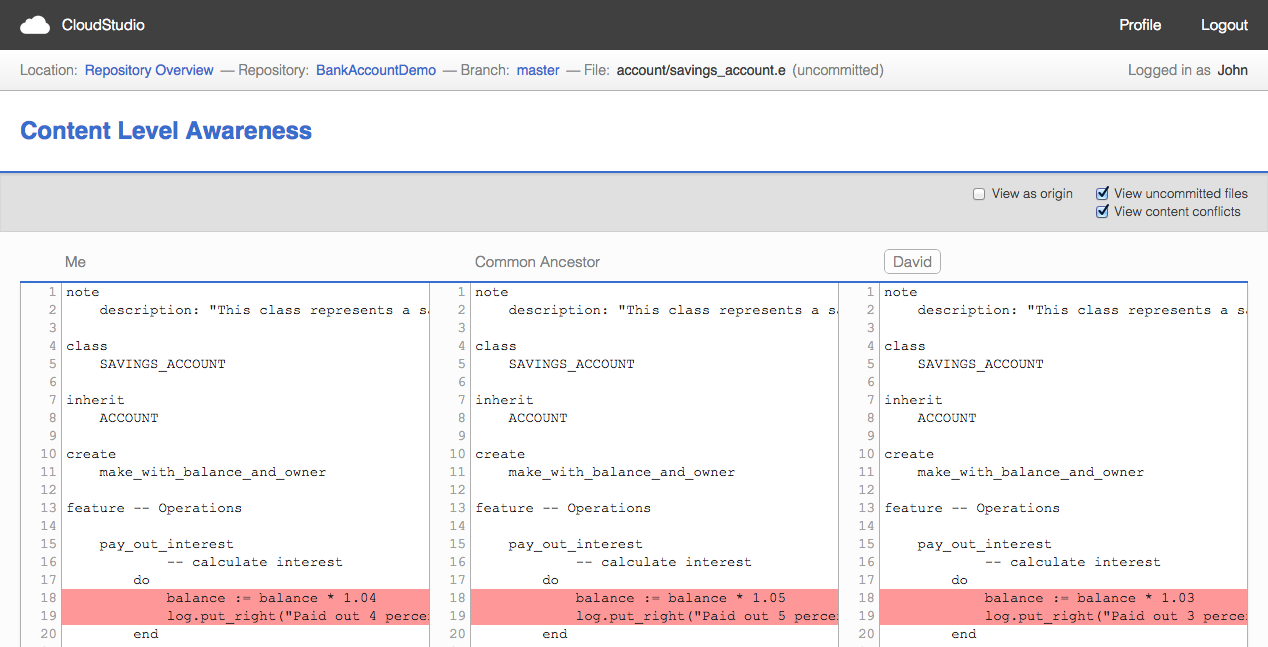
\includegraphics[width=0.9\textwidth]{contentlevel}}
  \caption{Web interface: content level awareness}
  \label{fig:contentlevel}
\end{figure}





\section{User Management}

Administrators can view users, manage their privileges, or delete their account altogether.






\begin{figure}[h!]
  \centering
  \frame{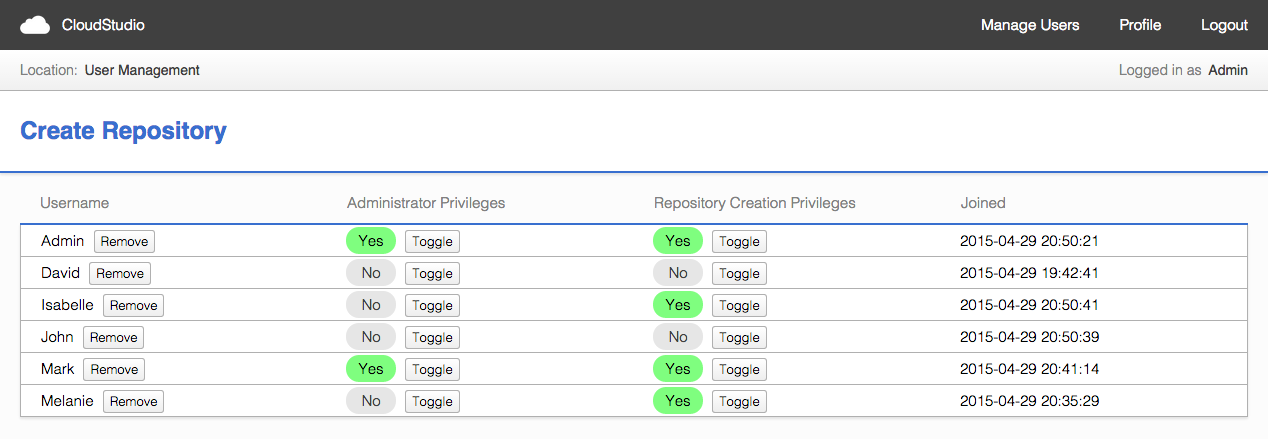
\includegraphics[width=0.9\textwidth]{manageusers}}
  \caption{User management}
  \label{fig:manageusers}
\end{figure}





\section{Create Repository}

This view lets you set up a new repository. The URL provided as remote repository will be periodically fetched by the CloudStudio server to make sure its data will be up to date.



\section{Edit Repository}

As an administrator or repository owner, this view lets you make modifications to its metadata, add or remove users, set a new repository owner or delete the repository altogether.

